% !TEX root = main.tex
%%%%%%%%%%%%%%%%%%%%%%%%%%%%%%%%%%%%%%%%%%%%%%%%%%%%%%
\section{実験システム}
%%%%%%%%%%%%%%%%%%%%%%%%%%%%%%%%%%%%%%%%%%%%%%%%%%%%%%
\subsection{構造}
 本研究では,図\ref{fig:system}に示すような模型を用いて実験を行う.
模型は,軸受を利用してできるだけ滑らかに回転し,各制御理論の特性がなるべく現れるようになっている.
台に乗っている物は,Arduino Uno,SD Cardシールド,センサ,回路,磁気トルカ,9V角型乾電池である.
Arduinoへの電力供給は角型乾電池を用い,磁気トルカへの電力供給は菊水電子工業株式会社のPMC18-5Aを用いる.
搭載した磁気トルカのパラメータを表\ref{table:torquer}に示す.
芯材であるPCパーマロイの選定理由は,その透磁率の高さである.PCパーマロイは比透磁率が約200,000で,磁気トルカがとらえられる磁力が高くなる.
なお,磁気トルカが発生させられるトルクは,磁気トルカの磁気モーメントを$\boldsymbol{M}$,磁気トルカがとらえる磁束を$\boldsymbol{B}$とすると,
\begin{equation}
	\boldsymbol{T = M \times B}
\end{equation}
とあらわされる.また,保磁力が低く,消磁しやすいため,必要な時だけトルクを発生させられる.
 表\ref{table:torquer}に示したものと同様のパラメータで芯材にステンレス鋼を用いて磁気トルカを作り,磁石を用いて反応性を確かめた.
しかし,ステンレス鋼の保磁力の高さのため,磁気トルカに電流を流していないときも磁力を持っており,
また比透磁率も低く,電流を流しているとき,いないときの差がなく磁力も低かったため,これを用いず
PCパーマロイを用いて磁気トルカの制作を行った.

\begin{table}[H]
	\centering
	\caption{磁気トルカのパラメータ}
	\label{table:torquer}
	\begin{tabular}{|c||c|}
		\hline
		コイル長さL [mm] & 100\\ \hline
		コイル直径D [mm] & 5\\ \hline
		巻き数n [-] & 983 \\ \hline
		インダクタンスL [mH] & 	82.017 \\ \hline
		抵抗 [$\Omega $] & 18.3 \\ \hline
		芯材 & PCパーマロイ \\ \hline
		線材 & ポリエステル被覆銅線 \\ \hline    
	\end{tabular}
\end{table}

 搭載するArduinoは,ELEGOO社のArduino Unoを,開発環境にはArduino IDEを用いた.
姿勢角度,角速度および磁力の検出には,Bosch Sensortec社のBNO055と,
Arduino IDEのライブラリ$"\mathrm{Adafruit\_Sensor.h}"$,$"\mathrm{Adafruit\_BNO055.h}"$
を用いる.また,姿勢角度,角速度および磁力の記録にはSDカードを用いており,
seeed studio社のSD Card shield V4.0をArduinoに装着している.
センサから取得した角度,角速度および磁気のデータを用いて,フィードバック制御を行う.
記録した角度・角速度のデータをCSVファイルに保存,それをPythonでグラフに描画し,姿勢角度の遷移を確認する.

\begin{figure}[H]
	\centering
		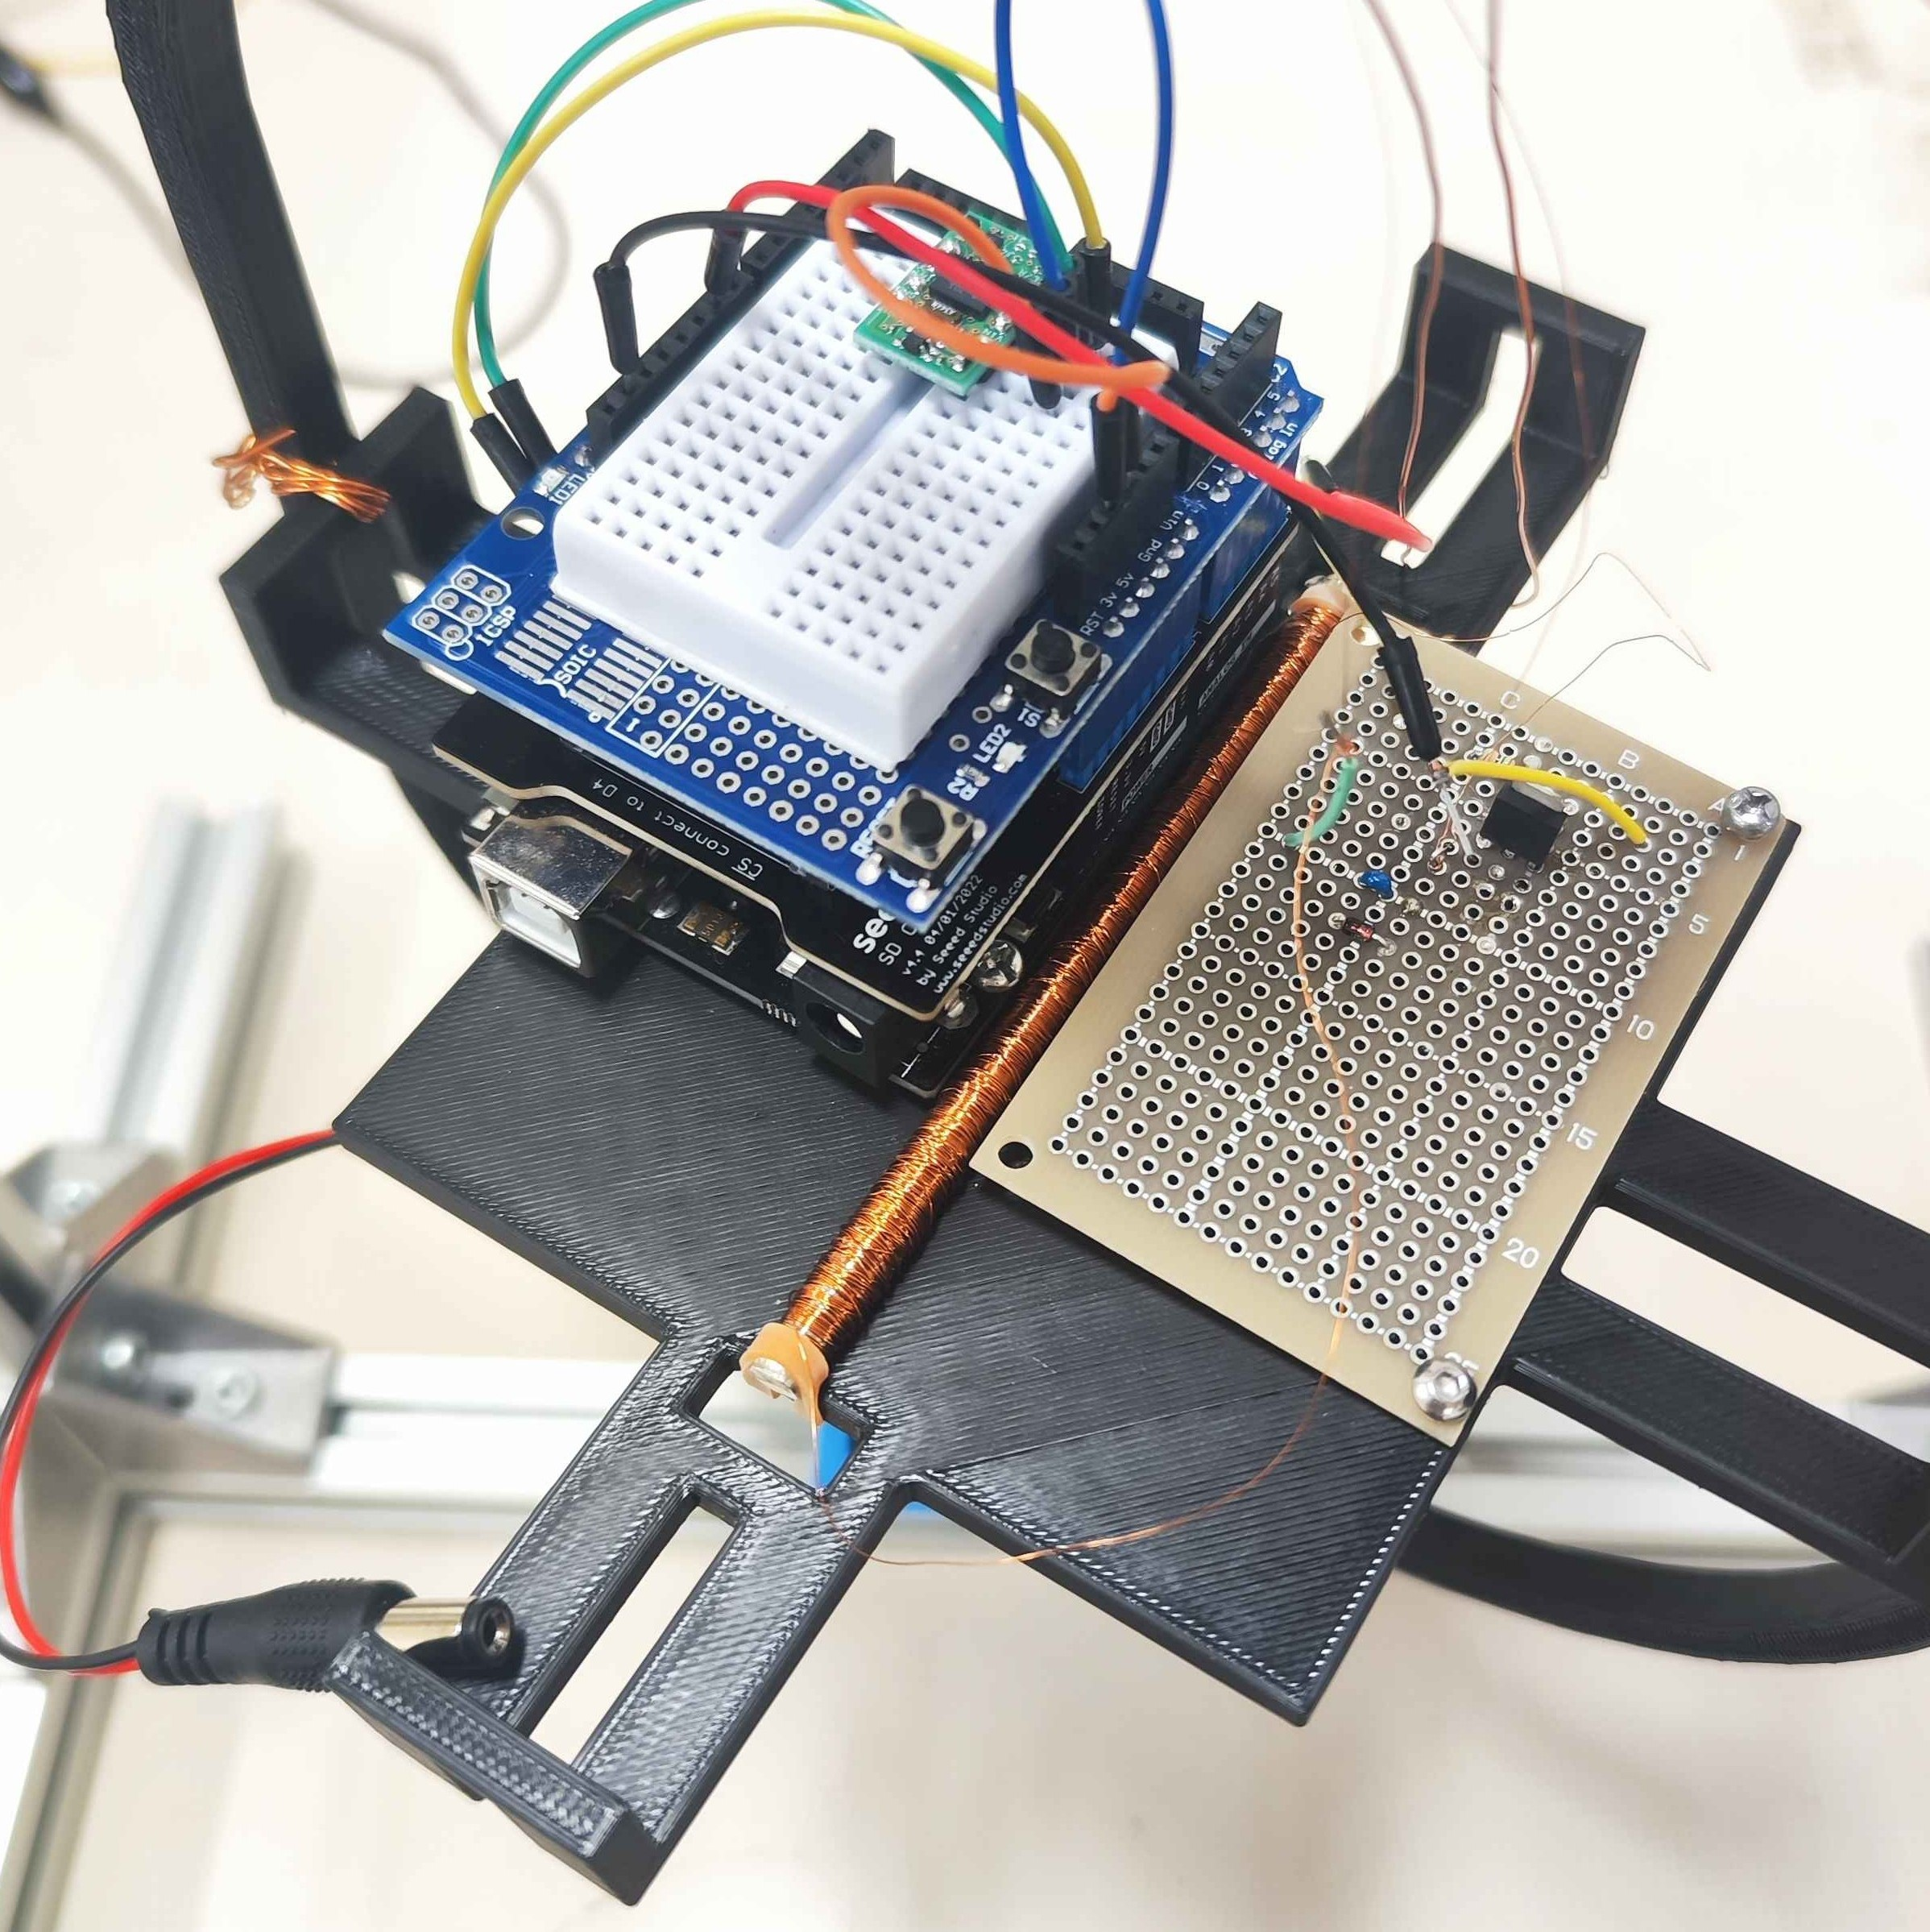
\includegraphics[scale=0.1]{./figure/実験システム.jpg}
		\caption{実験システム}
		\label{fig:system}
\end{figure}

\begin{figure}[H]
	\centering
		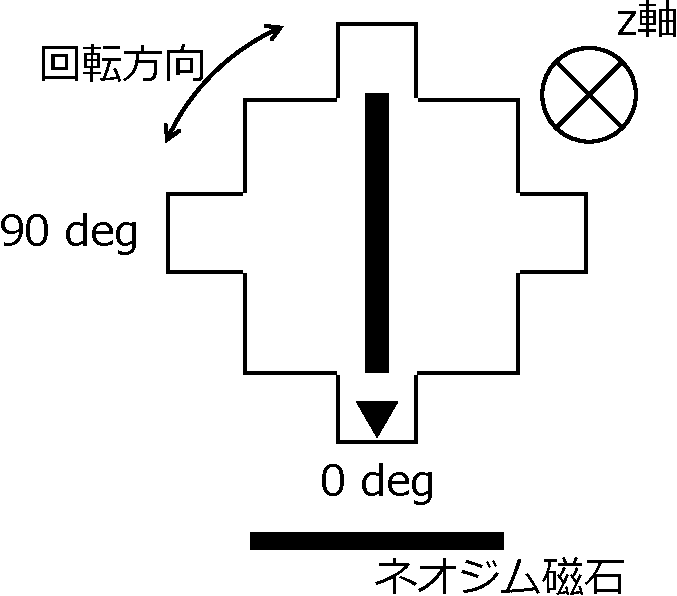
\includegraphics[scale=0.5]{./figure/system-crop.pdf}
		\caption{実験システム概略図}
		\label{fig:systemfig}
\end{figure}

%%%%%%%%%%%%%%%%%%%%%%%%%%%%%%%%%%%%%%%%%%%%%%%%%%%%%%
\subsection{回路構成}
%%%%%%%%%%%%%%%%%%%%%%%%%%%%%%%%%%%%%%%%%%%%%%%%%%%%%%
 図\ref{fig:cirkit1}に,最初に構築した回路図を示す.
この回路で,duty比50\%のPWM信号を入力した場合の,磁気トルカにかかる電圧を図\ref{fig:osiro1}に示す.
図\ref{fig:osiro1}のとおり,磁気トルカの逆起電力が大きい.
そのため,FETがOFFのとき,磁気トルカに流れる電流が本来流すべき方向と逆方向に流れ,逆方向のトルクが発生することが
予測された.

\begin{figure}[H]
	\centering
		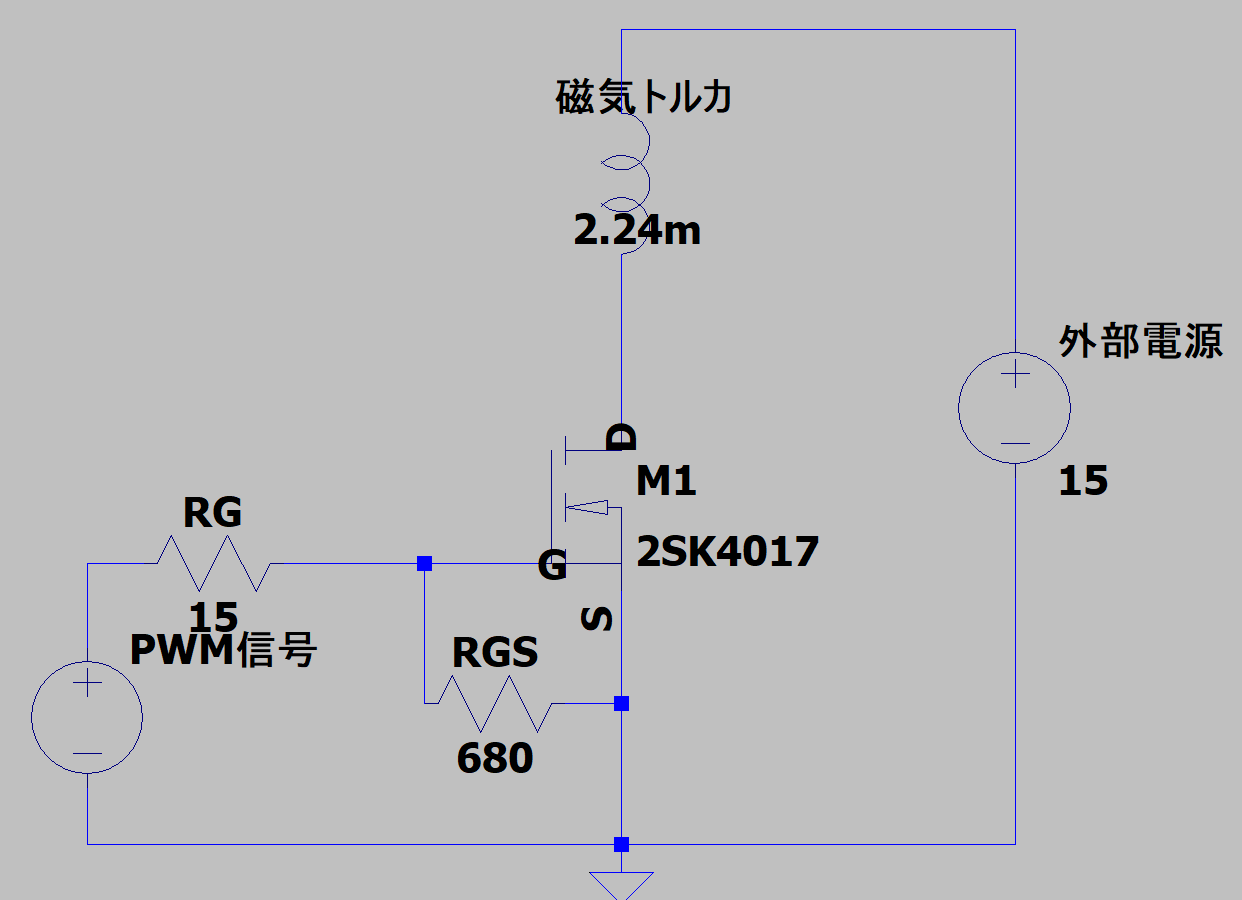
\includegraphics[scale=0.3]{./figure/回路図1.png}
		\caption{実験システムの回路図1}
		\label{fig:cirkit1}
\end{figure}

\begin{figure}[H]
	\centering
		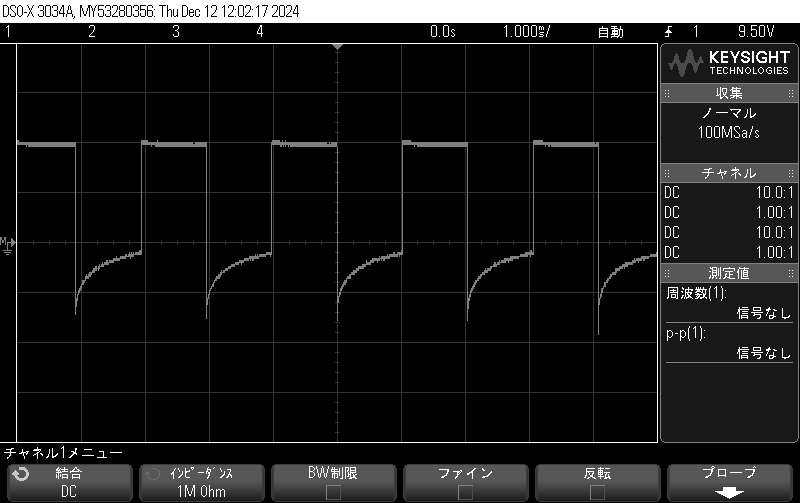
\includegraphics[scale=0.3]{./figure/scope_5.png}
		\caption{初期案}
		\label{fig:osiro1}
\end{figure}


 そこで次に,磁気トルカと並列にダイオードを接続することで逆起電力を防止した.
制作した回路の回路図を図\ref{fig:cirkit}に示す.
具体的には,ON時に磁気トルカに蓄えられたエネルギーを,
ダイオードを通して閉回路となった磁気トルカの抵抗により消費することにより,逆起電力を防ぐ.

 電流の制御をPWMで行うため,コイルの過渡特性を考慮して電流値の計算を行う必要がある.
一般的にコイルは,インダクタ成分のみでなく抵抗成分も含んでおり,低周波での等価回路は図\ref{fig:touka}のようになる.
よって,LR直列回路の過渡現象を考えればよい.
外部電源の電圧値$E=15$ [V],抵抗成分$R_L=18.3[\Omega]$,インダクタンス$L$ [mH] から求められるFETがONのときの電流の過渡特性は,

\begin{equation}
	i(t) = \frac{E}{R_L}\left(1-e^{-\frac{R_L}{L}t}\right)
\end{equation}

で表される.また,FETがOFFとなったときの時刻を$t_1$ [s] とすると,その後の電流の過渡特性は,

\begin{equation}
	i(t) = \frac{E\left(1-e^{-\frac{R_L}{L}t_1}\right)}{R_L}e^{-\frac{R_L}{L}(t-t_1)}
\end{equation}

となる.さらに$t_2$ [s] 経過すると,

\begin{equation}
	i(t) = \frac{E\left(1-e^{-\frac{R_L}{L}t_1}\right)e^{-\frac{R_L}{L}(t-t_1)}}{R_L}\left(1-e^{-\frac{R_L}{L}(t-t_1-t_2)}\right)
\end{equation}

というような電流の推移をする.この電流の推移を,図\ref{fig:cirkit}の回路を用いてduty比50\%でシミュレーションしたグラフを図\ref{fig:current50}に示す.
このように,磁気トルカに電圧E [V] を印加したときの電流を$I_\mathrm{max} [A]$とすると,duty比DのPWM信号で磁気トルカを駆動させたとき,
およその電流を$I(\mathrm{D})=I_\mathrm{max}D [A]$で近似できる                   . 

\begin{figure}[H]
	\centering
		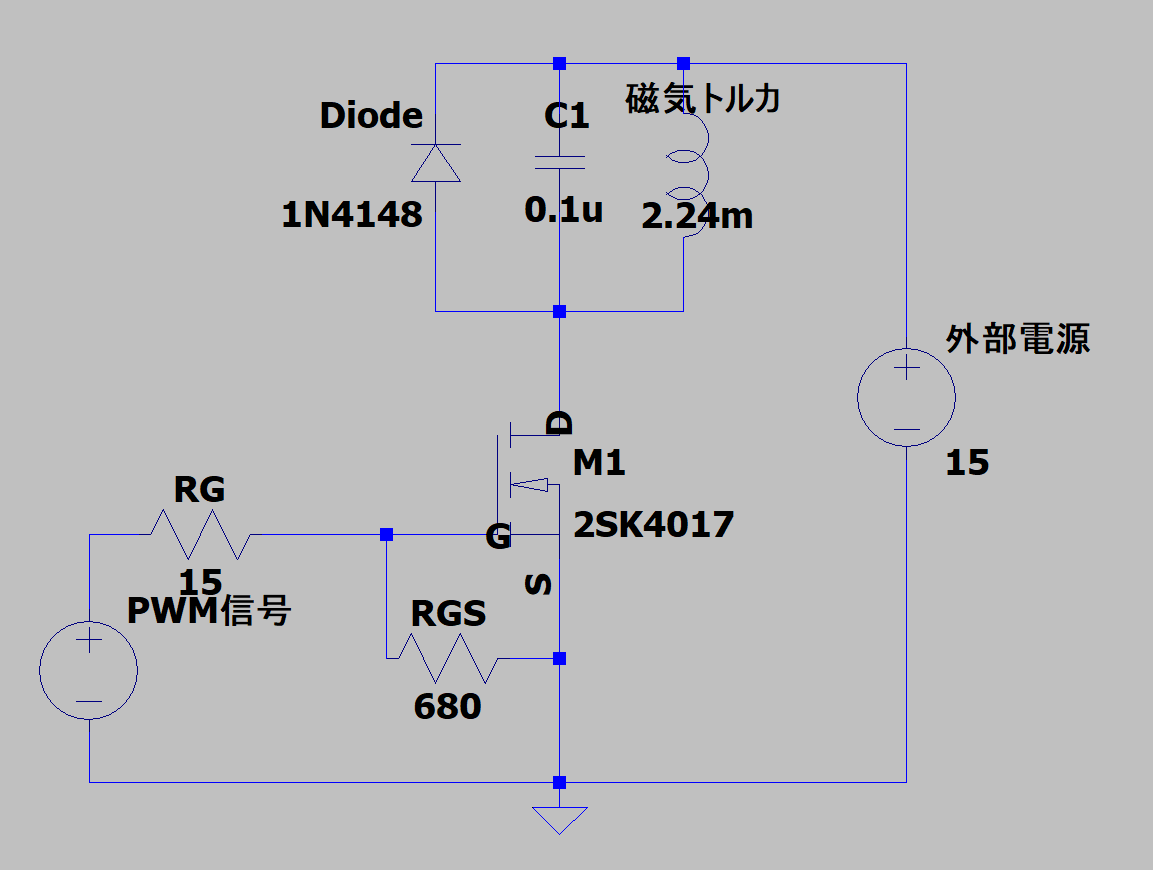
\includegraphics[scale=0.3]{./figure/回路図.png}
		\caption{実験システムの回路図}
		\label{fig:cirkit}
\end{figure}

\begin{figure}[H]
	\centering
		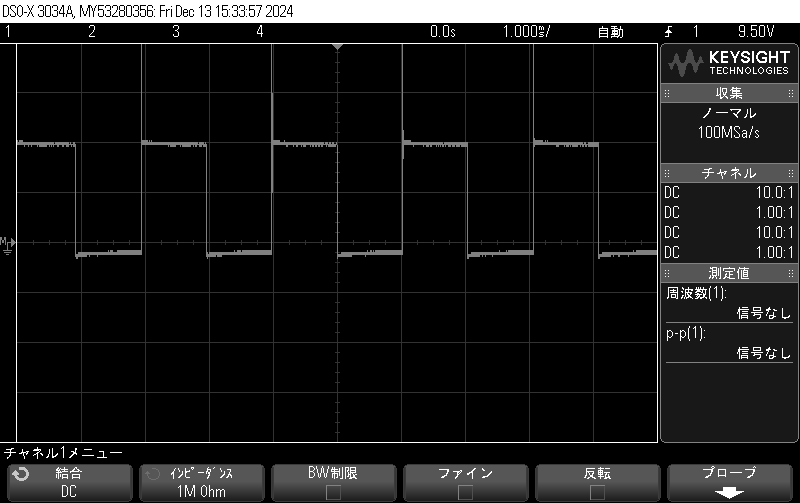
\includegraphics[scale=0.3]{./figure/scope_11.png}
		\caption{磁気トルカに加わる電圧}
		\label{fig:osiro2}
\end{figure}

\begin{figure}[H]
	\centering
		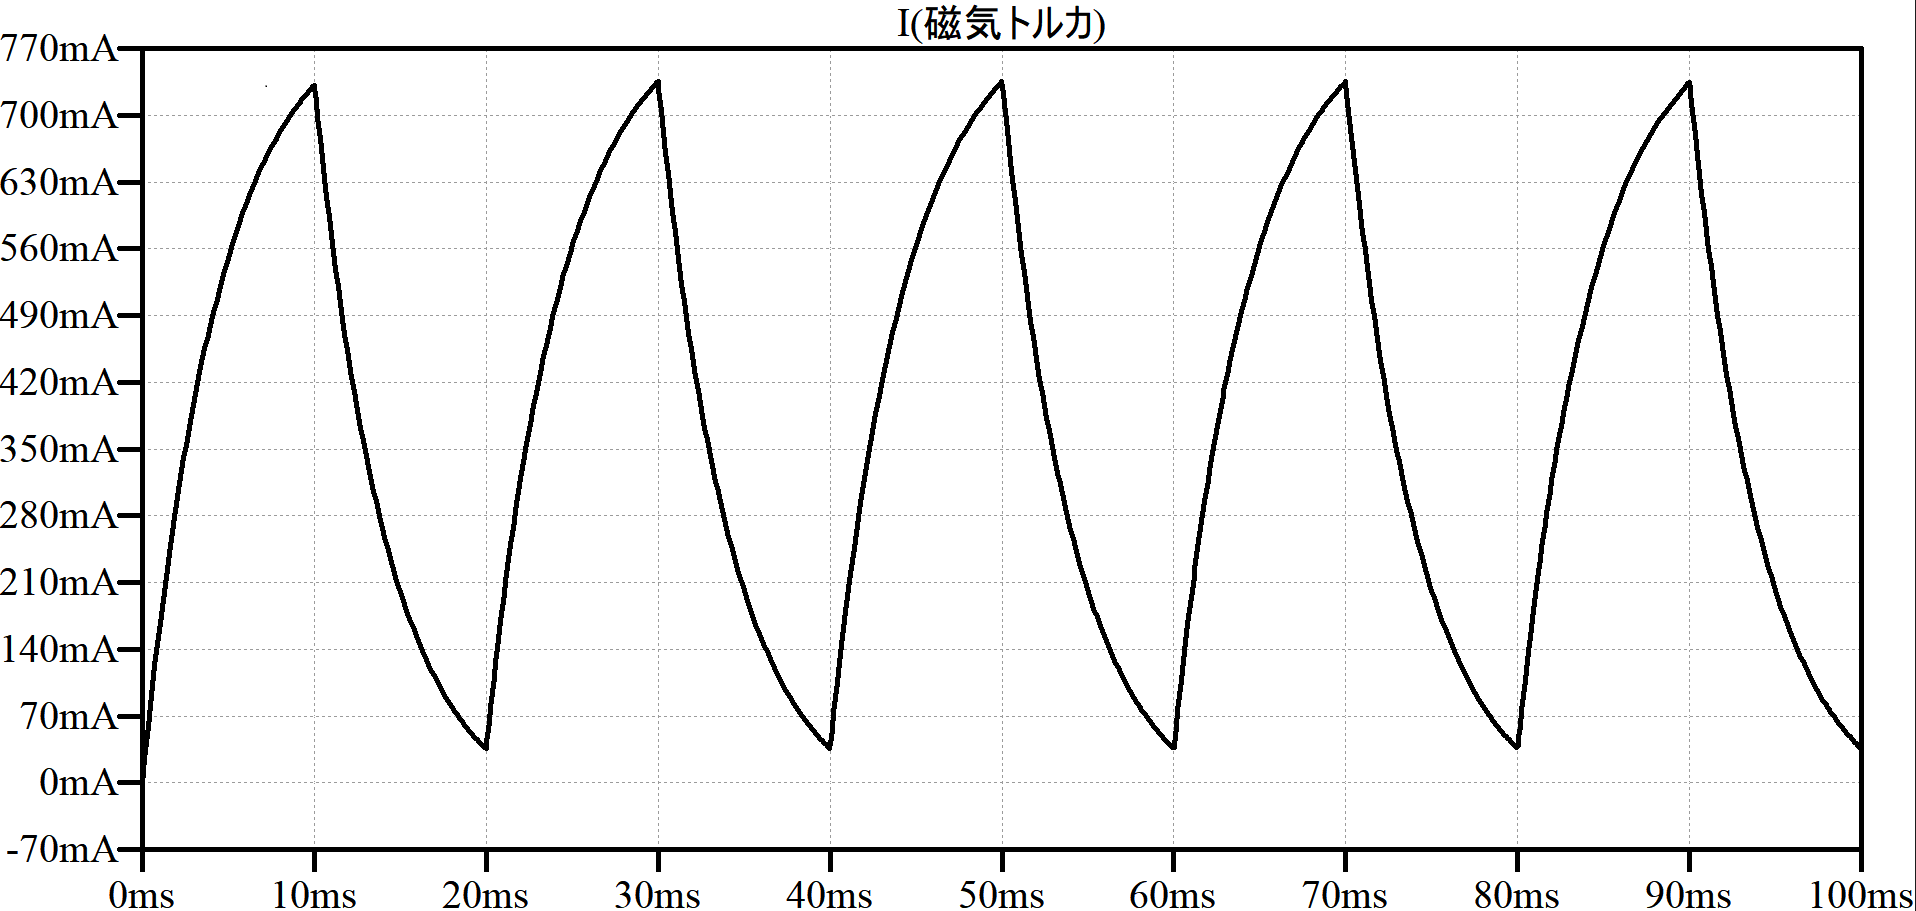
\includegraphics[scale=0.3]{./figure/50current.png}
		\caption{磁気トルカに加わる電圧}
		\label{fig:current50}
\end{figure}

\begin{figure}[H]
	\centering
		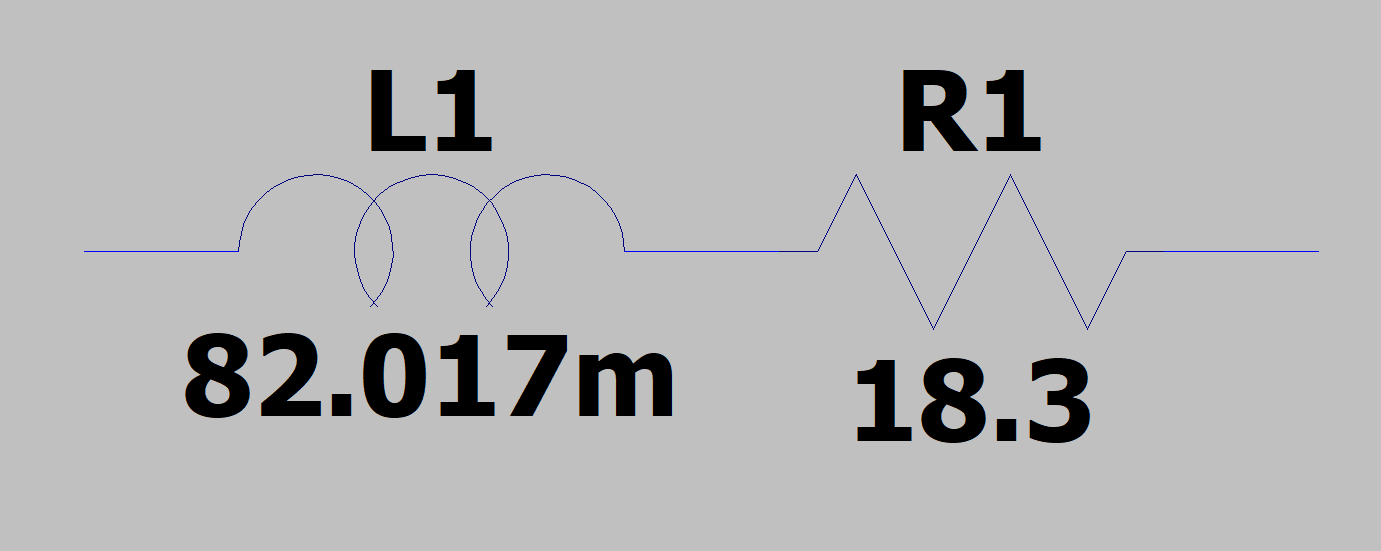
\includegraphics[scale=0.3]{./figure/touka.png}
		\caption{磁気トルカの等価回路}
		\label{fig:touka}
\end{figure}